% !Mode:: "TeX:UTF-8"
% !TEX root = ../main.tex

\section{Test Fonts 测试字体}

\subsection{字体集 Fontset}

\subsubsection{小标题 Heading3}

自动字体:普通,\verb|\textbf| \textbf{粗体},\verb|\textit| \textit{意大利斜体},\verb|\textsl| \textsl{倾斜体}

单独字体:{\songti 宋体},{\heiti 黑体},{\kaiti 楷体}
,{\fangsong 仿宋}% Ubuntu没有仿宋
% ,{\lishu 隶书},{\youyuan 幼圆}, % windows、founder和macnew中有隶书、幼圆
% ,{\yahei 微软雅黑} % windows中另有微软雅黑
% ,{\pingfang 苹方} % macnew另有苹方

Pandoc转义字体:\textbf{粗体},\verb|\emph| \emph{斜体},\verb|\sout| \sout{删除线}

English Text, \textbf{Bold English Text}, \textit{Italic English Text}

\subsection{带圈数字}

Unicode:
⓪ ① ② ③ ④ ⑤ ⑥ ⑦ ⑧ ⑨ ⑩ ⑪	⑫ ⑬	⑭ ⑮	⑯ ⑰ ⑱ ⑲	⑳ ㉑ ㉒	㉓ ㉔ ㉕ ㉖ ㉗ ㉘ ㉙ ㉚ ㉛ ㉜ ㉝ ㉞	㉟ ㊱ ㊲ ㊳ ㊴ ㊵ ㊶ ㊷ ㊸ ㊹ ㊺	㊻ ㊼ ㊽ ㊾ ㊿ 

\verb|\textcirciled{}|:
\textcircled{5} \textcircled{10} \textcircled{19} \textcircled{20} \textcircled{25} , \textcircled{56} \textcircled{87}  \textcircled{190}

圈码在正文中(检测基线平齐):

⑲ 榷盐院是官府垄断食盐产销的专门机构。其通常做法,是向盐户牧盐(即民制官收),再将盐税加入卖价,售予商人,听其运销,所过州县不再征税\footnote{宝坻县志编修委员会. 宝坻县志. 第一编, 建置区划, 置县. 天津社会科学院出版社. 1995-05, 第89页.};

⑳ 燕云一十六州:即幽、蓟、瀛、莫、涿、檀、顺、新、妫、儒、武、云、应、寰、朔、蔚州,相当于以今北京和大同为中心,东至河北遵化,北迄长城,西界山西神池,南至天津、河间、保定及山西繁峙、宁武一线以北地区\footnote{宝坻县志编修委员会. 宝坻县志. 第一编, 建置区划, 置县. 天津社会科学院出版社. 1995-05, 第89页.};

% \subsection{TH-Times\footnote{见\url{http://cheonhyeong.com/Tools/Times.html}}特色}
\subsection[TH-Times特色]{TH-Times{\protect\footnote{见\url{http://cheonhyeong.com/Tools/Times.html}}}特色}
音标:{\fb tʃi˥˧/ʈʂɨ˥˧ },西文 {\fb Бао-ди},


零宽附标 {\fb j+ü᪻̄=jū},环绕附标 {\fb Щ⃣ ​}

\subsubsection*{语言本地化:}

英语 {\fb rahîm M̧ajeļ gá}
, 土耳其语
% \begin{selectlanguage}{turkish}
    {\fbtk rahîm M̧ajeļ gá}
% \end{selectlanguage}
, 马绍尔语不适配
% \begin{selectlanguage}{marshallese}
    {rahîm M̧ajeļ gá}
% \end{selectlanguage}
, 简体中文
% \begin{selectlanguage}{chinese}
    {\fbcn rahîm M̧ajeļ gá}
% \end{selectlanguage}

简体中文{\fbcn 🀆 🀐 🩠 🩩},日本{\fbjp 🀆 🀐 🩠 🩩}

TH-Times定义为CJK字体:简体中文~文字{\fbcn ,}文字{\fbcn 、}\; 台湾繁体~{\cjktw 文字}{\fbpunctw ,}{\cjktw 文字}{\fbpunctw 、}

直接用NotoCJK对应字体:简体中文~{\cjkcn 文字,文字、}\; 台湾繁体~{\cjktw 文字,文字、}

\subsection{测试连字}

\noindent main字体:

\begin{quote}
    AE ae OE oe ff fi fl ij st ft et fs ffi ffl fa fe fo fr fb fh fu fy ch ct Qu Th mistake 2nd
\end{quote}


\noindent TH-Times字体:

\begin{quote}
    {\fb AE ae OE oe ff fi fl ij st ft et fs ffi ffl fa fe fo fr fb fh fu fy ch ct Qu Th mistake 2nd 2th 12th 12nd física Schiff‌fahrt Schieſ‍splat‍z}
\end{quote}


\noindent 插入ZWNJ \verb|\char"200C{}| 以停止连字:

\begin{quote}
    {\fb A\char"200C{}E a\char"200Ce O\char"200C{}E o\char"200Ce f\char"200Cf f\char"200Ci f\char"200Cl i\char"200Cj s\char"200Ct f\char"200Ct e\char"200Ct f\char"200Cs f\char"200Cf\char"200Ci f\char"200Cf\char"200Cl f\char"200Ca f\char"200Ce f\char"200Co f\char"200Cr f\char"200Cb f\char"200Ch f\char"200Cu f\char"200Cy c\char"200Ch c\char"200Ct Q\char"200Cu T\char"200Ch mis\char"200Ctake 2\char"200Cnd}
\end{quote}


\noindent 五度标记法连字 {\fb ˥˩˨˦˧˥˩˨˦˧˥˩˨˦˧, ꜔꜓꜕꜖꜒꜔꜓꜕꜖꜒꜔꜓꜕꜖꜒}

\subsection{变体字符}


蒙古文同一字母存在独立、字首、字中、字尾形式的不同变体,使用自由变体选择符(FVS,\verb|"180B、"180C、"180D|)实现。
八思巴文(1269年~1368年)有6个字母存在反转形式变体,使用标准变体序列(SVS,VS01 \verb|"FE00|)实现,以上见表\ref{tab:svs}。另八思巴文有4个元音存在位置变体,由字体引擎处理,见表\ref{tab:my_label}。


\begin{table}[!ht]
    \caption{Mongolian variants tests}
    \centering
    \begin{tabular}{llll}
    \hline
        预期字形 & 显示 & 变形类型 & 测试内容 \\ \hline
        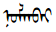
\includegraphics[height=1em]{figures/nomlabai.png} & \mongolianfont{ᠨᠣᠮ‍ᠯᠠᠪᠠᠢ} & 非强制 & 带有ZWJ的历史连字  \\ 
        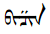
\includegraphics[height=1em]{figures/bischin.png} & \mongolianfont{ᠪᠢᡸᠢᠨ} & 强制 & U+1878能否为变形引擎所支持  \\ 
        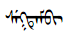
\includegraphics[height=1em]{figures/sektembi.png} & \mongolianfont{ᠰᡝᡴ᠏ᡨᡝᠮᠪᡳ} & 强制 & U+180F能否为变形引擎所支持  \\ 
        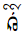
\includegraphics[height=1em]{figures/go.png} & \mongolianfont{ᡬᢅᠣ} & 强制 & baluda附标归位  \\ 
        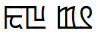
\includegraphics[height=1em]{figures/ttatthi.png} & \psp{ꡩꡖ︀ ꡪꡞ} & 强制 & 梵语镜像字母变形及SVS \\ \hline
    \end{tabular}
    \label{tab:svs}
\end{table}

\begin{table}[htbp]
    \caption{Test Phags-pa positional variants}
    \centering
    \begin{tabular}{rcccc}
        \hline
         & Isolate & Initial & Medial & Final\\
         \hline
        mainfont & ꡞ & ꡞꡄ & ꡄꡞꡄ & ꡄꡞ\\
        TH-Times default & {\fb ꡞ} & {\fb ꡞꡄ} & {\fb ꡄꡞꡄ} & {\fb ꡄꡞ}\\
        \verb|Script=Phags-pa| font & {\psp ꡞ} & {\psp ꡞꡄ} & {\psp ꡄꡞꡄ} & {\psp ꡄꡞ}\\
        \hline
    \end{tabular}
    \label{tab:my_label}
\end{table}

彩色字体 {\fb TH-Fonts,🐱🐶 2️⃣ 🀄︎🀄️ 🀐󠁊󠁐󠁿 🩠󠁋󠁒󠁿 🩩󠁋󠁒󠁿 🀢 🩬 R☖,\par 🀔 + ZWJ(\verb|\char"200D|)+ 🟥 以显示红宝牌: 🀔\char"200D🟥 🀝‍🟥 🀋\char"200D🟥}

\subsection{CJK兼容区测试}

U+F90x	豈	更	車	賈	滑	串	句	龜	龜	契	金	喇	奈	懶	癩	羅

U+F91x	蘿	螺	裸	邏	樂	洛	烙	珞	落	酪	駱	亂	卵	欄	爛	蘭

U+F92x	鸞	嵐	濫	藍	襤	拉	臘	蠟	廊	朗	浪	狼	郎	來	冷	勞

U+F93x	擄	櫓	爐	盧	老	蘆	虜	路	露	魯	鷺	碌	祿	綠	菉	錄

U+F94x	鹿	論	壟	弄	籠	聾	牢	磊	賂	雷	壘	屢	樓	淚	漏	累

U+F95x	縷	陋	勒	肋	凜	凌	稜	綾	菱	陵	讀	拏	樂	諾	丹	寧

U+F96x	怒	率	異	北	磻	便	復	不	泌	數	索	參	塞	省	葉	說

U+F97x	殺	辰	沈	拾	若	掠	略	亮	兩	凉	梁	糧	良	諒	量	勵

U+F98x	呂	女	廬	旅	濾	礪	閭	驪	麗	黎	力	曆	歷	轢	年	憐

U+F99x	戀	撚	漣	煉	璉	秊	練	聯	輦	蓮	連	鍊	列	劣	咽	烈

U+F9Ax	裂	說	廉	念	捻	殮	簾	獵	令	囹	寧	嶺	怜	玲	瑩	羚

U+F9Bx	聆	鈴	零	靈	領	例	禮	醴	隸	惡	了	僚	寮	尿	料	樂

U+F9Cx	燎	療	蓼	遼	龍	暈	阮	劉	杻	柳	流	溜	琉	留	硫	紐

U+F9Dx	類	六	戮	陸	倫	崙	淪	輪	律	慄	栗	率	隆	利	吏	履

U+F9Ex	易	李	梨	泥	理	痢	罹	裏	裡	里	離	匿	溺	吝	燐	璘

U+F9Fx	藺	隣	鱗	麟	林	淋	臨	立	笠	粒	狀	炙	識	什	茶	刺

U+FA0x	切	度	拓	糖	宅	洞	暴	輻	行	降	見	廓	兀	嗀	﨎	﨏

U+FA1x	塚	﨑	晴	﨓	﨔	凞	猪	益	礼	神	祥	福	靖	精	羽	﨟

U+FA2x	蘒	﨡	諸	﨣	﨤	逸	都	﨧	﨨	﨩	飯	飼	館	鶴	郞	隷

U+FA3x	侮	僧	免	勉	勤	卑	喝	嘆	器	塀	墨	層	屮	悔	慨	憎

U+FA4x	懲	敏	既	暑	梅	海	渚	漢	煮	爫	琢	碑	社	祉	祈	祐

U+FA5x	祖	祝	禍	禎	穀	突	節	練	縉	繁	署	者	臭	艹	艹	著

U+FA6x	褐	視	謁	謹	賓	贈	辶	逸	難	響	頻	恵	𤋮	舘		

U+FA7x	並	况	全	侀	充	冀	勇	勺	喝	啕	喙	嗢	塚	墳	奄	奔

U+FA8x	婢	嬨	廒	廙	彩	徭	惘	慎	愈	憎	慠	懲	戴	揄	搜	摒

U+FA9x	敖	晴	朗	望	杖	歹	殺	流	滛	滋	漢	瀞	煮	瞧	爵	犯

U+FAAx	猪	瑱	甆	画	瘝	瘟	益	盛	直	睊	着	磌	窱	節	类	絛

U+FABx	練	缾	者	荒	華	蝹	襁	覆	視	調	諸	請	謁	諾	諭	謹

U+FACx	變	贈	輸	遲	醙	鉶	陼	難	靖	韛	響	頋	頻	鬒	龜	𢡊

U+FADx	𢡄	𣏕	㮝	䀘	䀹	𥉉	𥳐	𧻓	齃	龎

